\section{Area-Loss Estimate}
\label{sec:area-loss}

The area-loss method records how much of each V triangle must lie outside
$H$.  The local estimate applies to every V triangle. A final cyclic argument
adds these losses without imposing a center type.

Put $A_\triangle=\sqrt3/4$ and normalize all areas by $A_\triangle$.  At
$V_0$ define
\[
 \mathcal T(a,b):=
 \left\{T:\begin{array}{l}
 T\text{ is a closed unit equilateral triangle},\\
 \{V_0,V_0+a(V_5-V_0),V_0+b(V_1-V_0)\}\subseteq T
 \end{array}\right\},
\]
\[
 \mathcal L(T):=\frac{\operatorname{area}(T\setminus H)}{A_\triangle},
 \qquad
 \mathcal L(a,b):=\inf_{T\in\mathcal T(a,b)}\mathcal L(T),
\]
where $a,b\in[0,1]$ and $\mathcal T(a,b)\ne\varnothing$.  Hexagon
symmetry gives the corresponding family at every $V_i$.  In particular,
if
\[
 0\le a_i\le A_i,
 \qquad
 0\le b_i\le B_i,
\]
then the rotated copy of $T_i$ belongs to $\mathcal T(a_i,b_i)$.

\begin{figure}[H]
\centering
\begin{minipage}[b]{.48\textwidth}
\centering
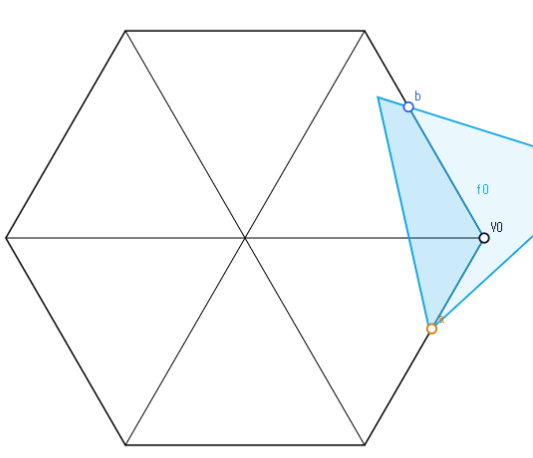
\includegraphics[width=\linewidth]
  {figures/strategy3_local_area_loss.png}
\par\smallskip
\footnotesize (a) local retained area
\end{minipage}\hfill
\begin{minipage}[b]{.48\textwidth}
\centering
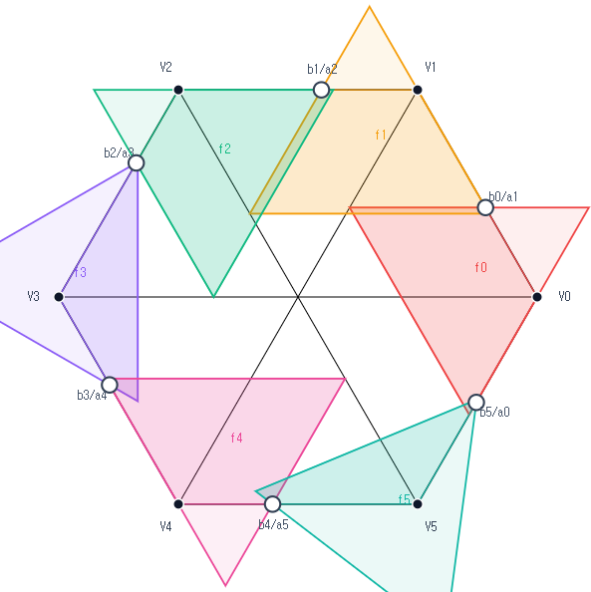
\includegraphics[width=\linewidth]
  {figures/strategy3_global_area_loss.png}
\par\smallskip
\footnotesize (b) cyclic retained areas
\end{minipage}
\caption{The area-loss method.  The dark regions indicate the portions
retained in $H$; the exact quantities are $\mathcal L(T)$ and
$\mathcal L(a,b)$.}
\label{fig:area-loss}
\end{figure}

\subsection{Local area loss}

\begin{theorem}[Local square loss]
\label{thm:local-square-loss}
For every feasible $(a,b)$,
\begin{equation}
 \mathcal L(a,b)\ge\min\{a,b\}^2.               \label{eq:min-square-loss}
\end{equation}
If $a+b>1$, then
\begin{equation}
 \mathcal L(a,b)\ge\max\{a,b\}^2.               \label{eq:max-square-loss}
\end{equation}
The same bounds hold for every $T\in\mathcal T(a,b)$.
\end{theorem}

\begin{proof}
The two exhaustive orientation families give these minima.  Their polygon
areas and the factorizations proving both inequalities are computed in
\zcref{lem:appendix-local-square-loss}.
\end{proof}

\subsection{Cyclic accumulation}

Use the strict handoffs from \zcref{prop:strict-handoffs}:
\[
 \xi_i\in(1-A_{i+1},B_i),
 \qquad
 a_i:=1-\xi_{i-1},
 \qquad
 b_i:=\xi_i.
\]
They satisfy
\[
 0<a_i<A_i,
 \qquad
 0<b_i<B_i,
 \qquad
 a_i^2+a_ib_i+b_i^2<1.
\]

\begin{lemma}[Cyclic area-loss certificate]
\label{lem:cyclic-area-loss}
The six actual V triangles satisfy
\[
 \left|\{i\in\mathbb Z/6\mathbb Z:a_i+b_i>1\}\right|\ge2
 \quad\Longrightarrow\quad
 \sum_{i=0}^5\mathcal L(T_i)>1.
\]
\end{lemma}

\begin{proof}
Apply the local bounds around the six-cycle.  The exact sum, including
the strict contribution from the second ascent, are given in
\zcref{lem:appendix-cyclic-area-loss}.
\end{proof}

\begin{proposition}[Branch closed by area]
\label{prop:area-branches}
The branch $N_{\rm gap}=0$, $N_+\ge2$ is impossible.
\end{proposition}
\begin{proof}
The six V triangles cover $\partial H$. The at-least-two clause of
\zcref{prop:strict-handoffs} supplies the selection for
\zcref{lem:cyclic-area-loss}. Thus the V triangles have total normalized
inside area below five. The C triangle contributes at most one, whereas
$H$ has normalized area six. Apply \zcref{lem:open-cover-budget} with area.
\end{proof}
